\chapter{Dritte Iteration}\label{chap:pro3}
\todo{Hauptaspekt in die Überschrift: Dritte Iteration - für eine intuitivere App-Nutzung}
Die beim Testen des zweiten Prototyps in \autoref{sec:test2} identifizierten Probleme sollen nun in einer dritten Iteration des \hcdp{} gelöst werden.
Hierzu werden, wie schon im vorherigen Abschnitt, die vier Phasen des Zyklus ein weiteres Mal durchlaufen.
Das Ziel dieses Kapitels ist es, durch die Entwicklung eines dritten Prototyps die Usability-Probleme aus dem Zweiten zu lösen, und die Anwenderwünsche aus dem vorherigen Kapitel umzusetzen.

\section{Observation}\label{sec:obs3}
Um auch in diesem Abschnitt einen Überblick über die gesammelten Test-Ergebnisse aus \autoref{sec:test2} zu bekommen, werden diese im Nachfolgenden zur Übersicht aufgelistet und anschließend weiter evaluiert:

\begin{enumerate}
  \item Hilfestellung beim initialen Start der App unzureichend
  \item Auswahlmöglichkeiten im Farbdialog zu fortgeschrittenen
  \item Gerüsttyp-Indikator nicht intuitiv als solcher erkennbar
  \item Kognitive Last beim Eintragen der Messwerte im Gerüsttyp-Dialog zu hoch
  \item Anwenderwunsch: Einführen einer Freitext-Form
  \item Anwenderwunsch: Einführen einer Pfeil-Form 
\end{enumerate}

\noindent
Die Testergebnisse zeigen, dass beide Testpersonen in \autoref{sec:test2} Nutzungsprobleme aufgrund einer unzureichenden Hilfestellung beim initialen Start der App gehabt haben.
Daher müssen Funktionen der App durch eine Art ``Trial and Error'' erkundet werden.
Dies erzeugt nicht nur einen negativen ersten Eindruck beim Nutzer, sondern potenziert das Auftreten von Situationen, in denen Fehler enstehen können.
Besonders diese beiden Punkte führen schnell zu einem negativen Anwendererlebnis der App, und erschweren somit bereits zu Beginn die Nutzung der App.
(Nielsen~\autoref{itm:N5} \& \autoref{itm:N13}) \\

Die zu fortgeschrittenen Auswahlmöglichkeiten im Farbdialog sind ein weiteres Usability-Problem, das sich während der Testphase in \autoref{sec:test2} gezeigt hat.
Durch die Verwendung eines Farbkreises, der das Auswählen einer beliebigen Farbe und der dazugehörigen Transparenz ermöglicht, zeigen sich beide Testpersonen überfordert.
Diese vielen Auswahlmöglichkeiten übertreffen das Ziel des Benutzers, der nur schnell und unkompliziert eine Farbe auszuwählen möchte.
(Nielsen~\autoref{itm:N12}) \\

Außerdem wird aus den Testergebnissen ersichtlich, dass der verwendete Indikator für die verlinkten Gerüsttypen nicht intuitiv als solcher erkennbar ist.
Die Benutzung einer einzelnen Zahl als Indikator für die Anzahl der verknüpften Gerüste zu einer Form hat nicht genug Wiedererkennungswert, um mit den Gerüsttypen assoziiert zu werden.
Hier fehlt ein wiedererkennbares Icon, welches dem Benutzer den Kontext des Indikators intuitiv vermittelt.
(Nielsen~\autoref{itm:N6}) \\

Zudem belasten die Eingabefelder im Gerüsttyp-Dialog die kognitiven Fähigkeiten der Testpersonen zu sehr.
Da die Eingabefelder keinerlei Vorschläge für die einzutragenden Werte bieten, müssen die Nutzer sich die Messwerte merken, welche sie anschließend in den Dialog eintragen wollen.
Dies führt im schlimmsten Fall dazu, dass mehrfach zwischen Dialog und Bild gewechselt werden muss, um alle Messwerte in den Dialog eintragen zu können.
Weil Dialoge unter Android standardmäßig nicht minimiert, und zu einem späteren Zeitpunkt wieder angezeigt werden können, ohne dass eingetragenen Informationen verloren gehen, muss der Benutzer alle zuvor eingetragenen Daten beim Schließen und wieder Öffnen des Dialogs erneut eingeben.
(Nielsen~\autoref{itm:N11}) \\

Zusätzlich zu den Usability-Problemen des zweiten Prototyps, die sich in \autoref{sec:test2} gezeigt haben, gab es Wünsche für neue Funktionen, die regelmäßig im Arbeitsalltag der Testpersonen gebraucht werden.
So soll die App um zwei neue Formen, der Freitext- und Pfeil-Form, erweitert werden.
Die Freitext-Form soll dem Nutzer ermöglichen, beliebige Texte auf das Bild zu schreiben, ohne zuvor eine Form zeichnen zu müssen. 
Durch die Pfeil-Form sollen Längen, die sich mit Hilfe der Linien-Form nicht gut abbilden lassen, dargestellt werden. \\

\section{Idea Generation}\label{sec:idea3}
\todo{Wie referenziere ich hier auf }
Um dem Benutzer beim Start der App einen Überblick über die beiden Modi und den darin enthaltenen Funktionen zu geben, soll eine Hilfestellung beim initialen Start der App angezeigt werden.
Die \mg{} suggerieren zur Umsetzung eines solchen ``Onboarding''-Prozesses\urlnote{https://material.io/guidelines/growth-communications/onboarding.html\#onboarding-onboarding-models} drei verschiedene Ansätze (vgl. \autoref{fig:onboarding}). \\

\begin{figure}[h]
  \centering
  \begin{subfigure}[t]{0.3\textwidth}
    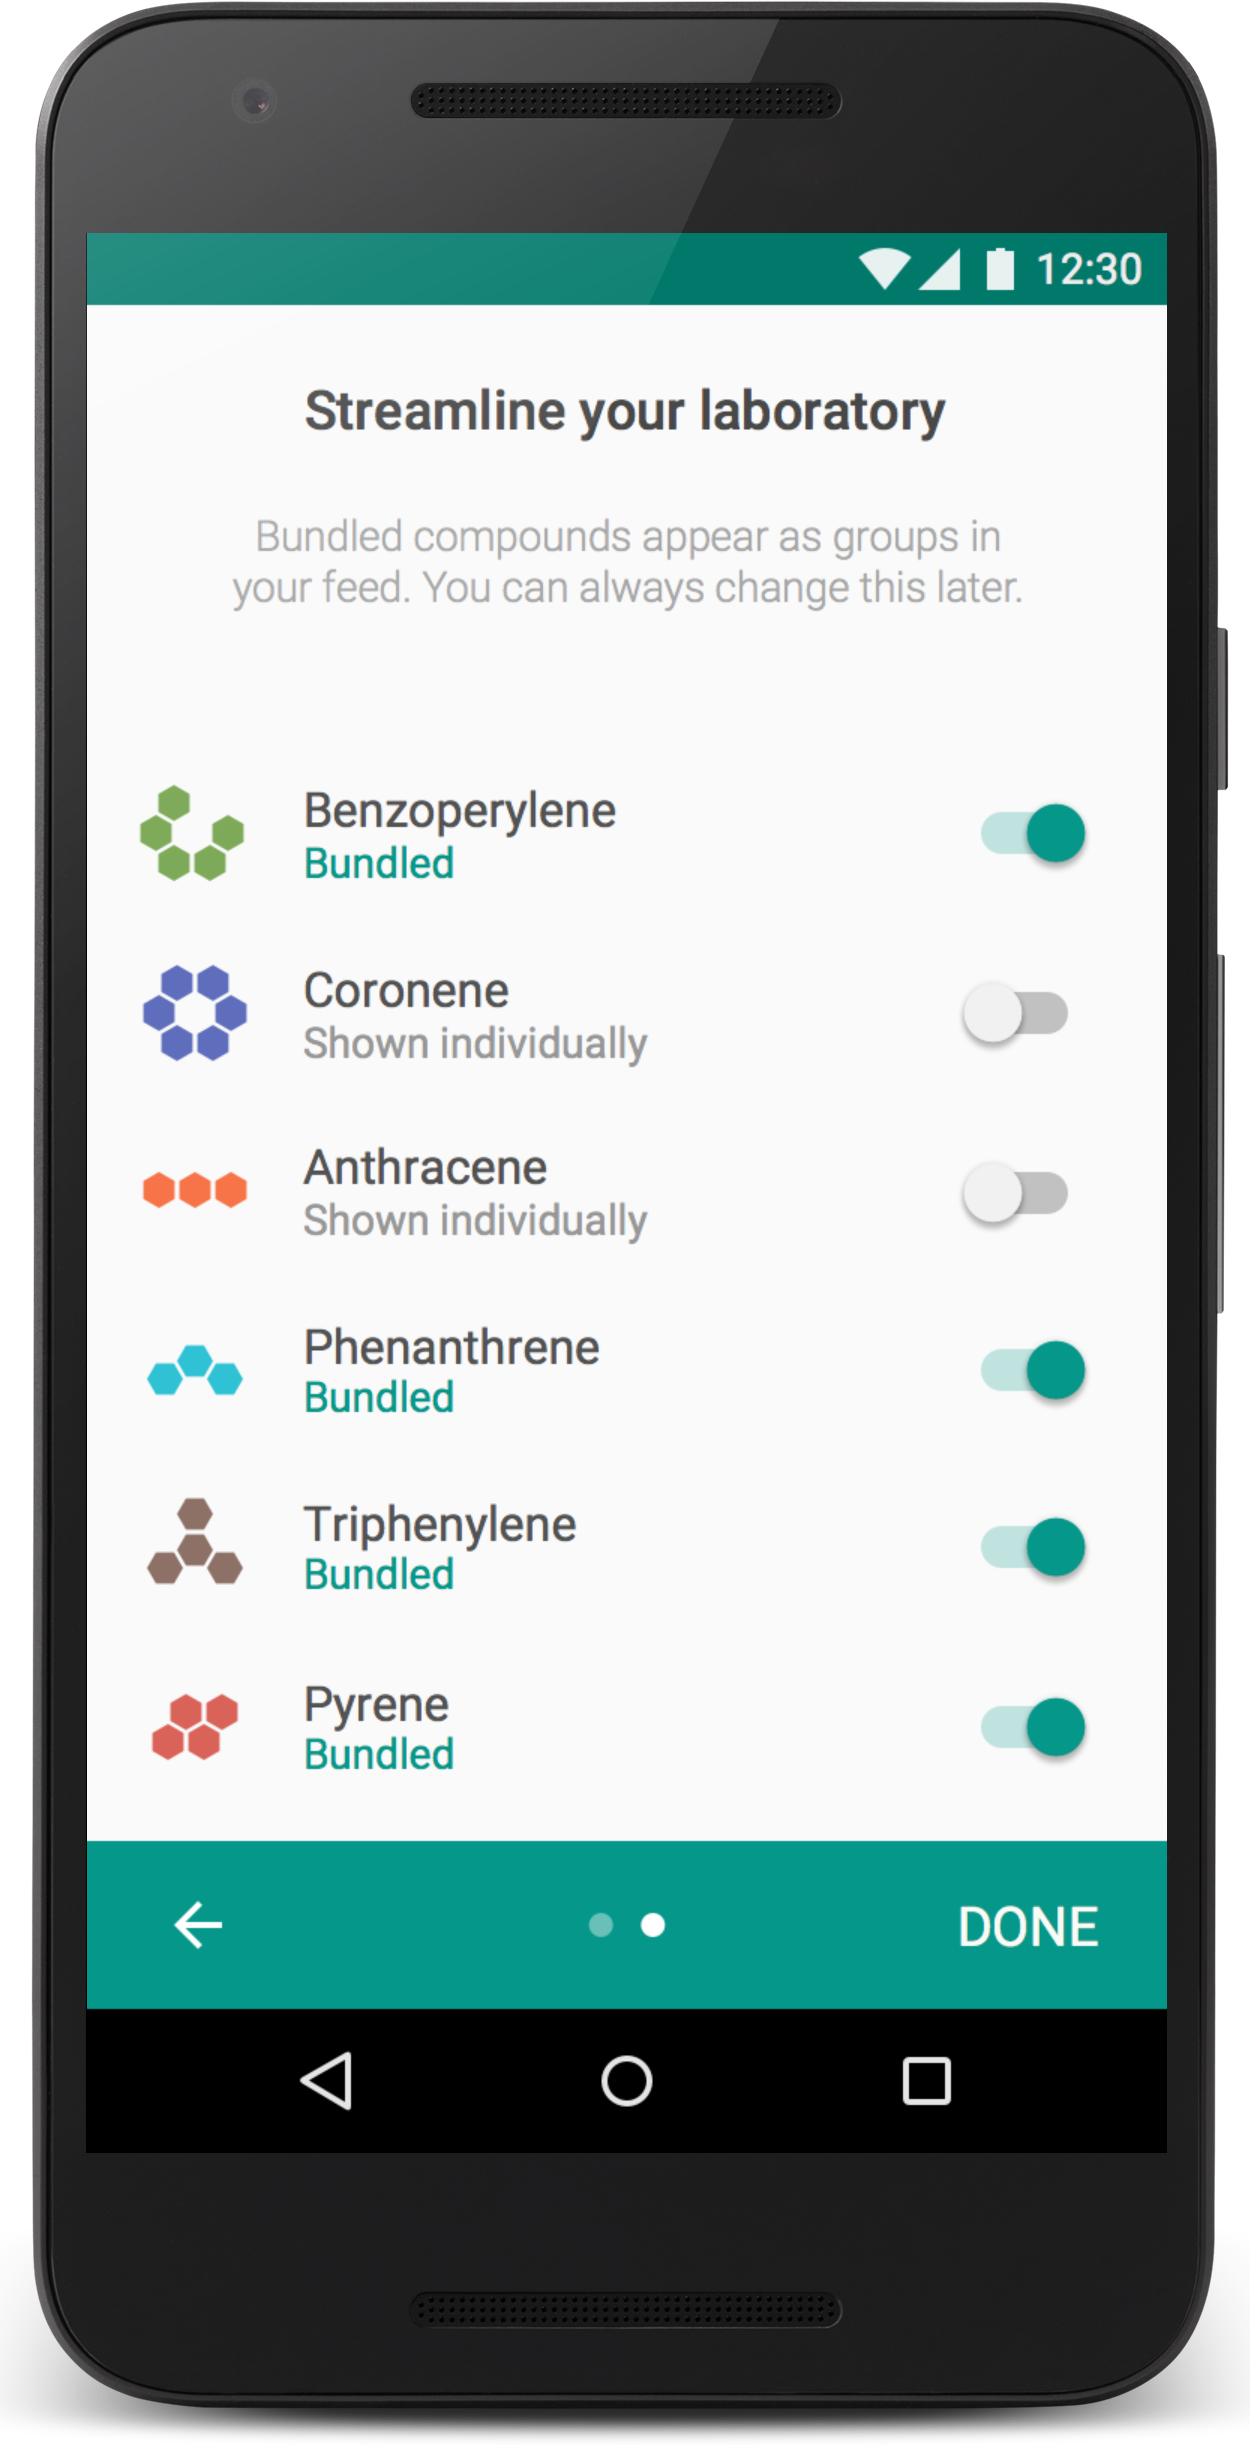
\includegraphics[keepaspectratio, width=\textwidth]{prototype3/selfselect}
    \caption{Selft-Select}
    \label{fig:selfselect}
  \end{subfigure}
  \begin{subfigure}[t]{0.3\textwidth}
    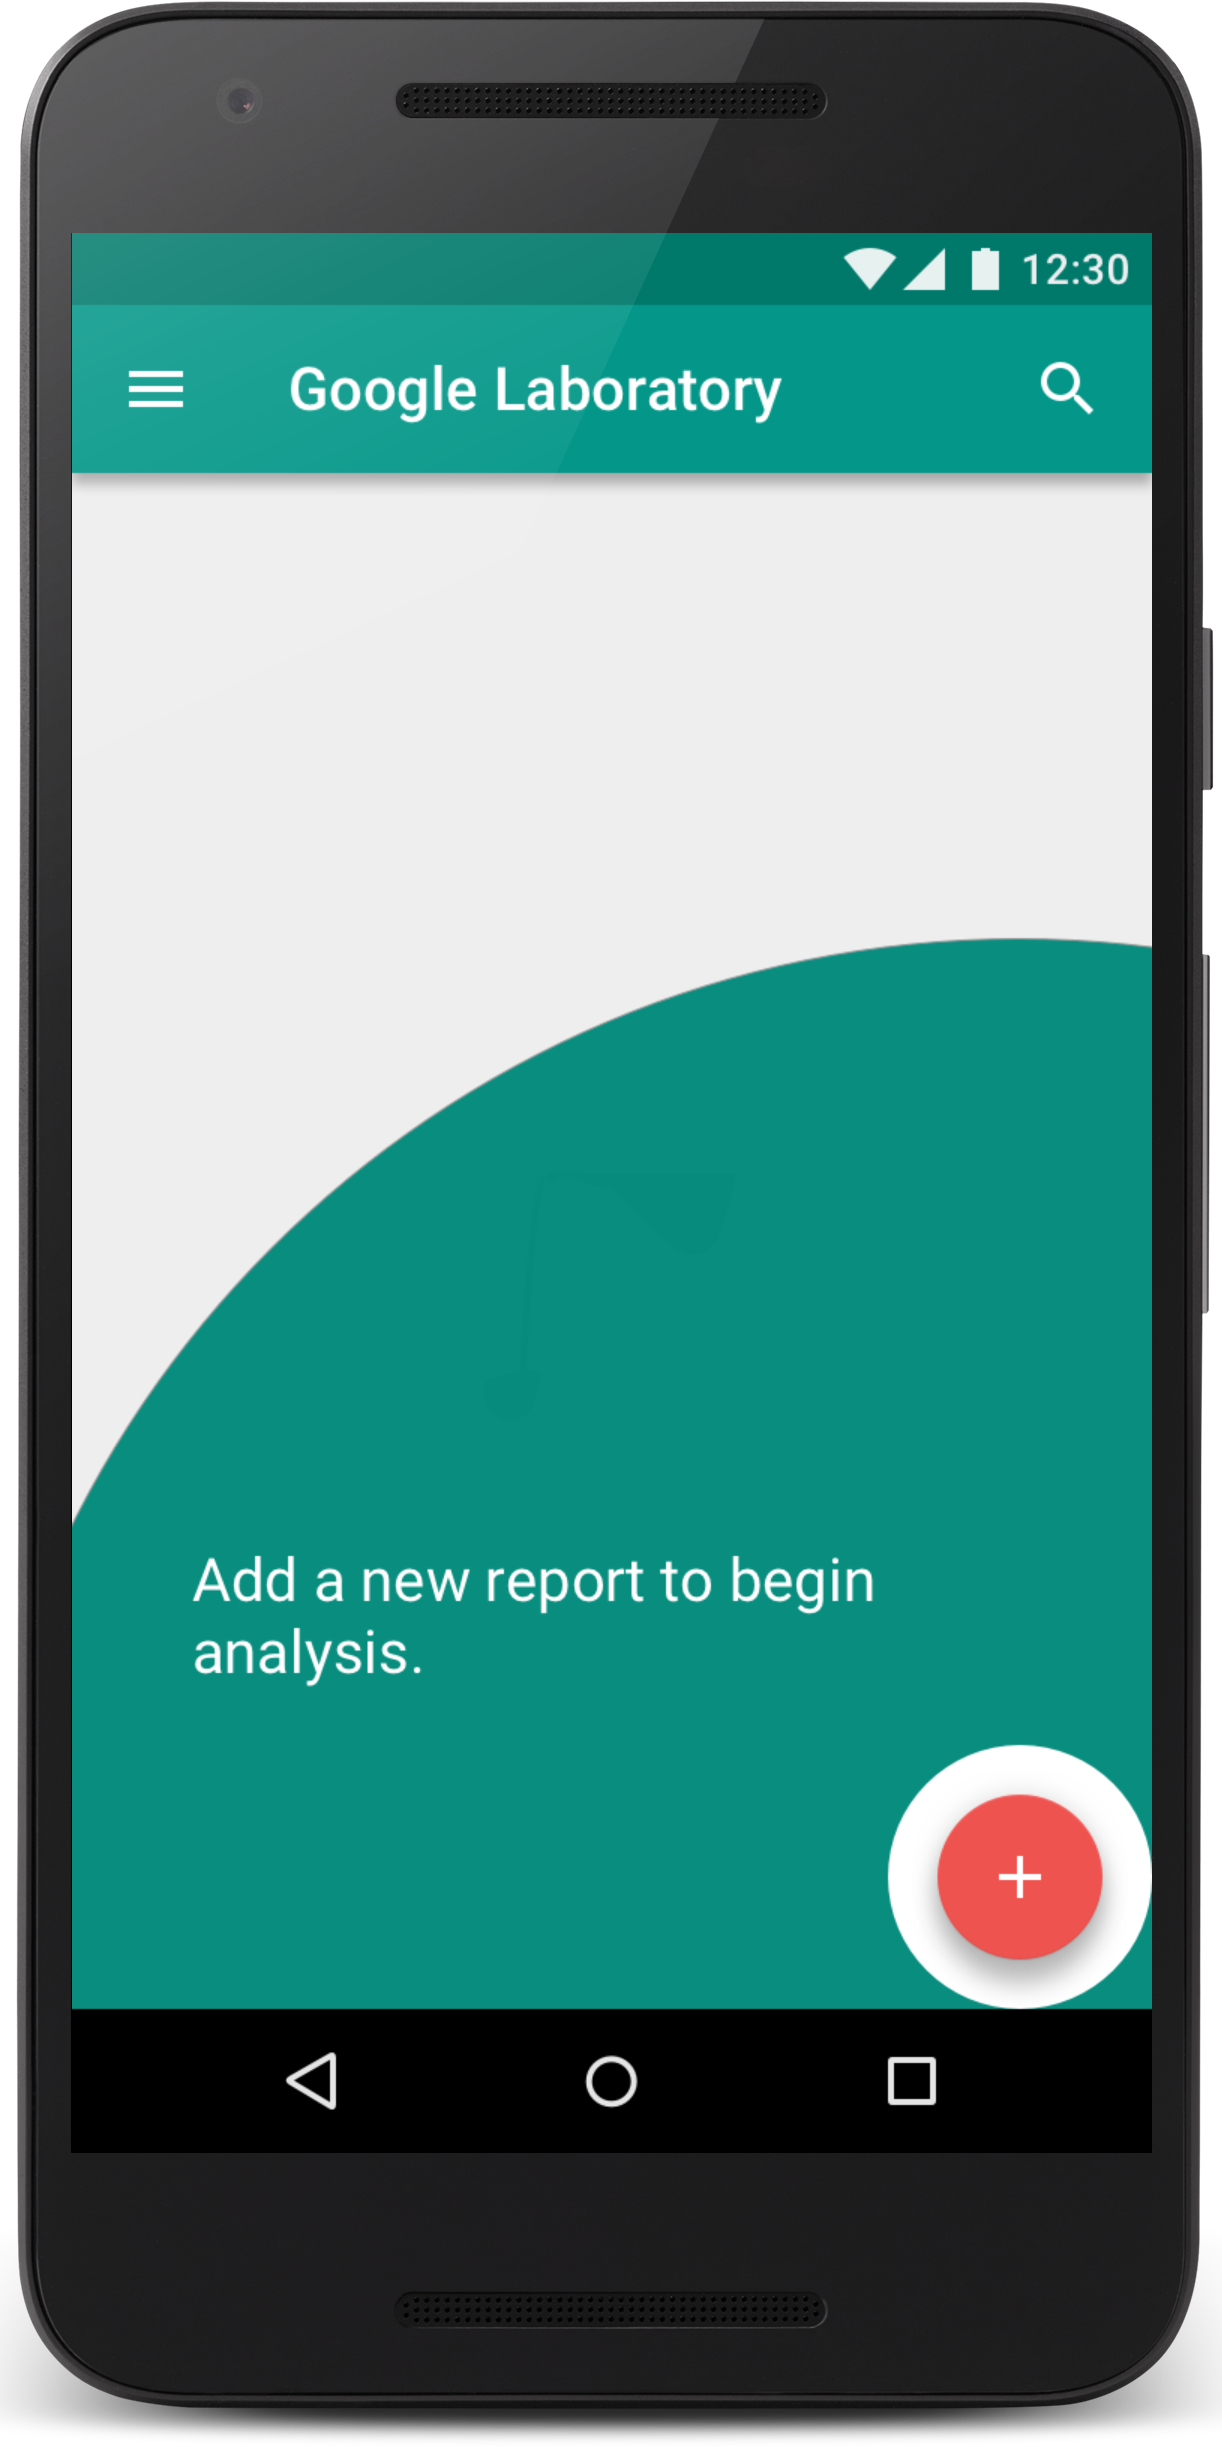
\includegraphics[keepaspectratio, width=\textwidth]{prototype3/quickstart}
    \caption{Quickstart}
    \label{fig:quickstart}
  \end{subfigure}
  \begin{subfigure}[t]{0.3\textwidth}
    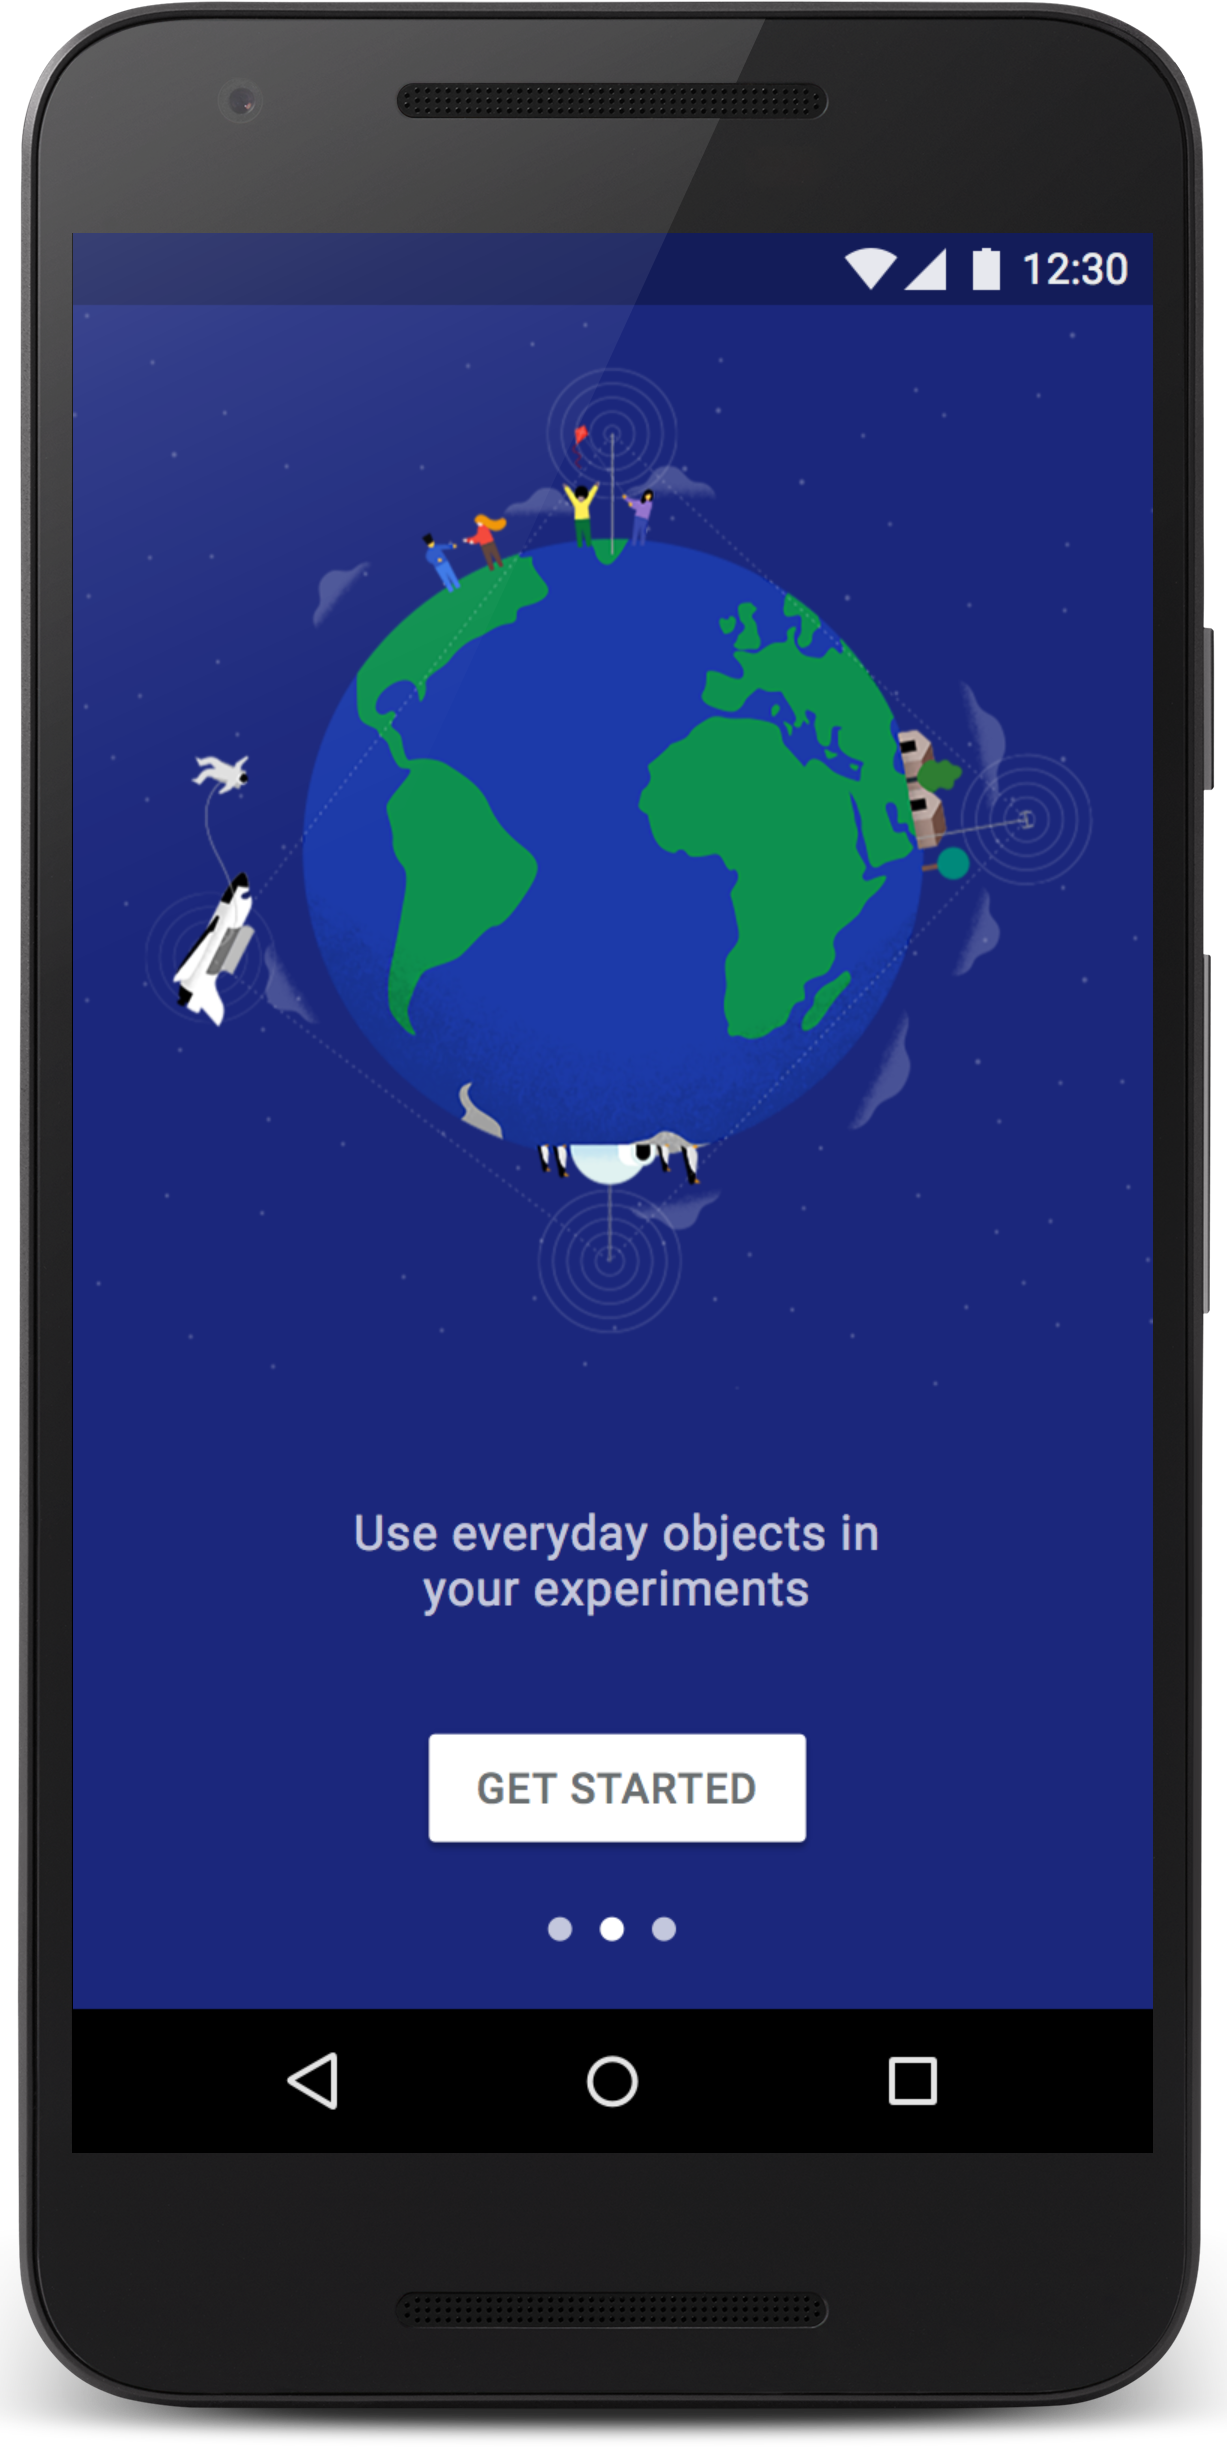
\includegraphics[keepaspectratio, width=\textwidth]{prototype3/userbenefits}
    \caption{Top User Benefits}
    \label{fig:benefits}
  \end{subfigure}
  \caption{Die drei verschiedenen ``Onboarding''-Ansätze nach den \mg{}}
  \label{fig:onboarding}
\end{figure}

Zu den drei ``Onboarding''-Ansätzen werden auch die jeweiligen ``Use-Cases'' angegeben, für die sich die Umsetzungsmöglichkeiten jeweils am Besten eignen \citep[Abschnitt ``Usage'']{Onboarding}.
So biete sich bspw. die \emph{Self-Select}-Variante (siehe \autoref{fig:selfselect}) dann an, wenn der Nutzer beim initialen Start der App bereits diverse Einstellungen konfigurieren muss.
Die \emph{Quickstart}-Variante (siehe \autoref{fig:quickstart}) solle, so die \mg{}, dann genutzt werden, wenn bereits identifiziert werden konnte, welche Funktionen der App besonders hervorgehoben werden soll.
Diese Funktion solle dem Nutzer dann beim initialen Start der App vorgestellt werden, und so als ``Call for action'' dienen.
Die Variante des \emph{Top User Benefits} (siehe \autoref{fig:benefits}) könne nach den \mg{} am besten dann sinnvoll eingesetzt werden, wenn neue Funktionalität oder große Änderungen der Benutzeroberfläche angekündigt werden sollen. \\

Damit der Farbdialog den Nutzer nicht mehr mit zu vielen Anpassungsmöglichkeiten überfordert, sollen diese auf ein Minimum reduziert werden.
So kann der Dialog bspw. so verändert werden, dass er nur eine Palette der häufigst genutzten Farben anzeigt, und auf die Einstellungsmöglichkeit der Transparenz ganz verzichtet.
Um die volle Breite des Farbkreises nicht zu verlieren, bietet es sich an, den fortgeschrittenen Modus, wie er im zweiten Prototyp standardmäßig angezeigt wird, über einen Button im Dialog zugänglich zu machen.
So kann der erfahrene Nutzer, falls er keine Farbe der Standardpalette benutzen möchte, über den fortgeschrittenen Modus eine beliebige Farbe und deren Transparenz auswählen. \\

Die Wiedererkennbarkeit des Gerüsttyp-Indikators könnte durch die Benutzung eines Icons neben der Indikator-Zahl verbessert werden.
Alternativ bietet es sich an, einen weiteren Text zum Indikator hinzuzufügen, der verdeutlicht, dass es sich bei der Indikator-Zahl um die Anzahl der verknüpften Gerüsttypen handelt.
Hierbei muss jedoch bei der praktischen Umsetzung darauf geachtet werden, dass nur eine begrenzte Menge Text auf dem Bildschirm gleichzeitig anzeigen werden sollte, bevor dieser zu unübersichtlich wird. \\

Um die kognitive Last der Nutzer beim Eintragen der Messwerte im Gerüsttyp-Dialog zu minimieren, bietet sich die Verwendung von Vorschlägen in den Eingabefeldern an.
Diese Vorschläge können dann z.B. aus den bereits hinterlegten Messwerten der jeweiligen Form stammen.
So hat der Nutzer zum Beispiel bei der Verlinkung einer Rechtecks-Form zu einem Gerüsttyp die Möglichkeit aus bis zu vier verschiedenen Vorschlägen (vier Kanten) auszuwählen.

Sowohl die Freitext- als auch die Pfeil-Form kann als Unterklasse der bestehenden abstrakten Oberklasse \emph{MeasureShape} modelliert werden.
Wichtig bei der Freitext-Form wird es sein, einen geeigneten Text-Hintergrund zu verwenden, damit der Text auch auf dunkleren Bildern ohne Anstrengung lesbar ist.
Hierzu bietet es sich an, die Ergebnisse aus \autoref{sec:idea2} bezüglich der Erkennbarkeit von eingetragenen Messwerten wiederzuverwenden.

\section{Prototyping}
Der dritte Prototyp wurde am 16. Januar 2018 in die bestehende Android-App eingebunden.
Bei der Implementierung dieses Prototyps wurde versucht alle in \autoref{sec:idea3} genannten Ideen zur Lösung der in \autoref{sec:obs3} identifizierten Probleme umzusetzen. \\

So wurde von den drei verschiedenen Ansatzmöglichkeiten zur Umsetzung des ``Onboarding''-Prozesses die Variante des \emph{Quickstarts} gewählt, da der ``Use-Case'' dieser am besten auf den Prototyp zutrifft.
Umgesetzt wurde die \emph{Quickstart} Variante mit Hilfe sogenannter \emph{Tap targets}\urlnote{https://material.io/guidelines/growth-communications/feature-discovery.html\#feature-discovery-design}.
Hiervon wurden insgesamt drei in den Prototyp integriert, welche jeweils an einer anderen Stelle dem Nutzer angezeigt werden (siehe \autoref{fig:taptargets}).
Ein \emph{Tap target} wird beim initialen Start der App angezeigt, und gibt dem Nutzer eine kurze Hilfestellung zu der \emph{Bottom bar} und dem damit verbundenen Zeichen- und Text-Modus (siehe \autoref{fig:helpmode}).
Die anderen beiden \emph{Tap targets} werden jeweils beim ersten Wechsel in den Text- bzw. Zeichen-Modus angezeigt, und beschreiben, welche Aktionen in dem jeweiligen Modus durchführbar sind (vgl. \autoref{fig:helpdraw} \& \autoref{fig:helptext}).
Die erklärenden Texte und auch die Position der einzelnen \emph{Tap targets} wurde so gewählt, dass der Nutzer die wichtigsten UI-Elemente der App fokussiert und über einen kurzen, aber präzisen Text alle wichtigen Informationen zur Benutzung dieser erhält. \\

\begin{figure}[h]
  \centering
  \begin{subfigure}[t]{0.3\textwidth}
    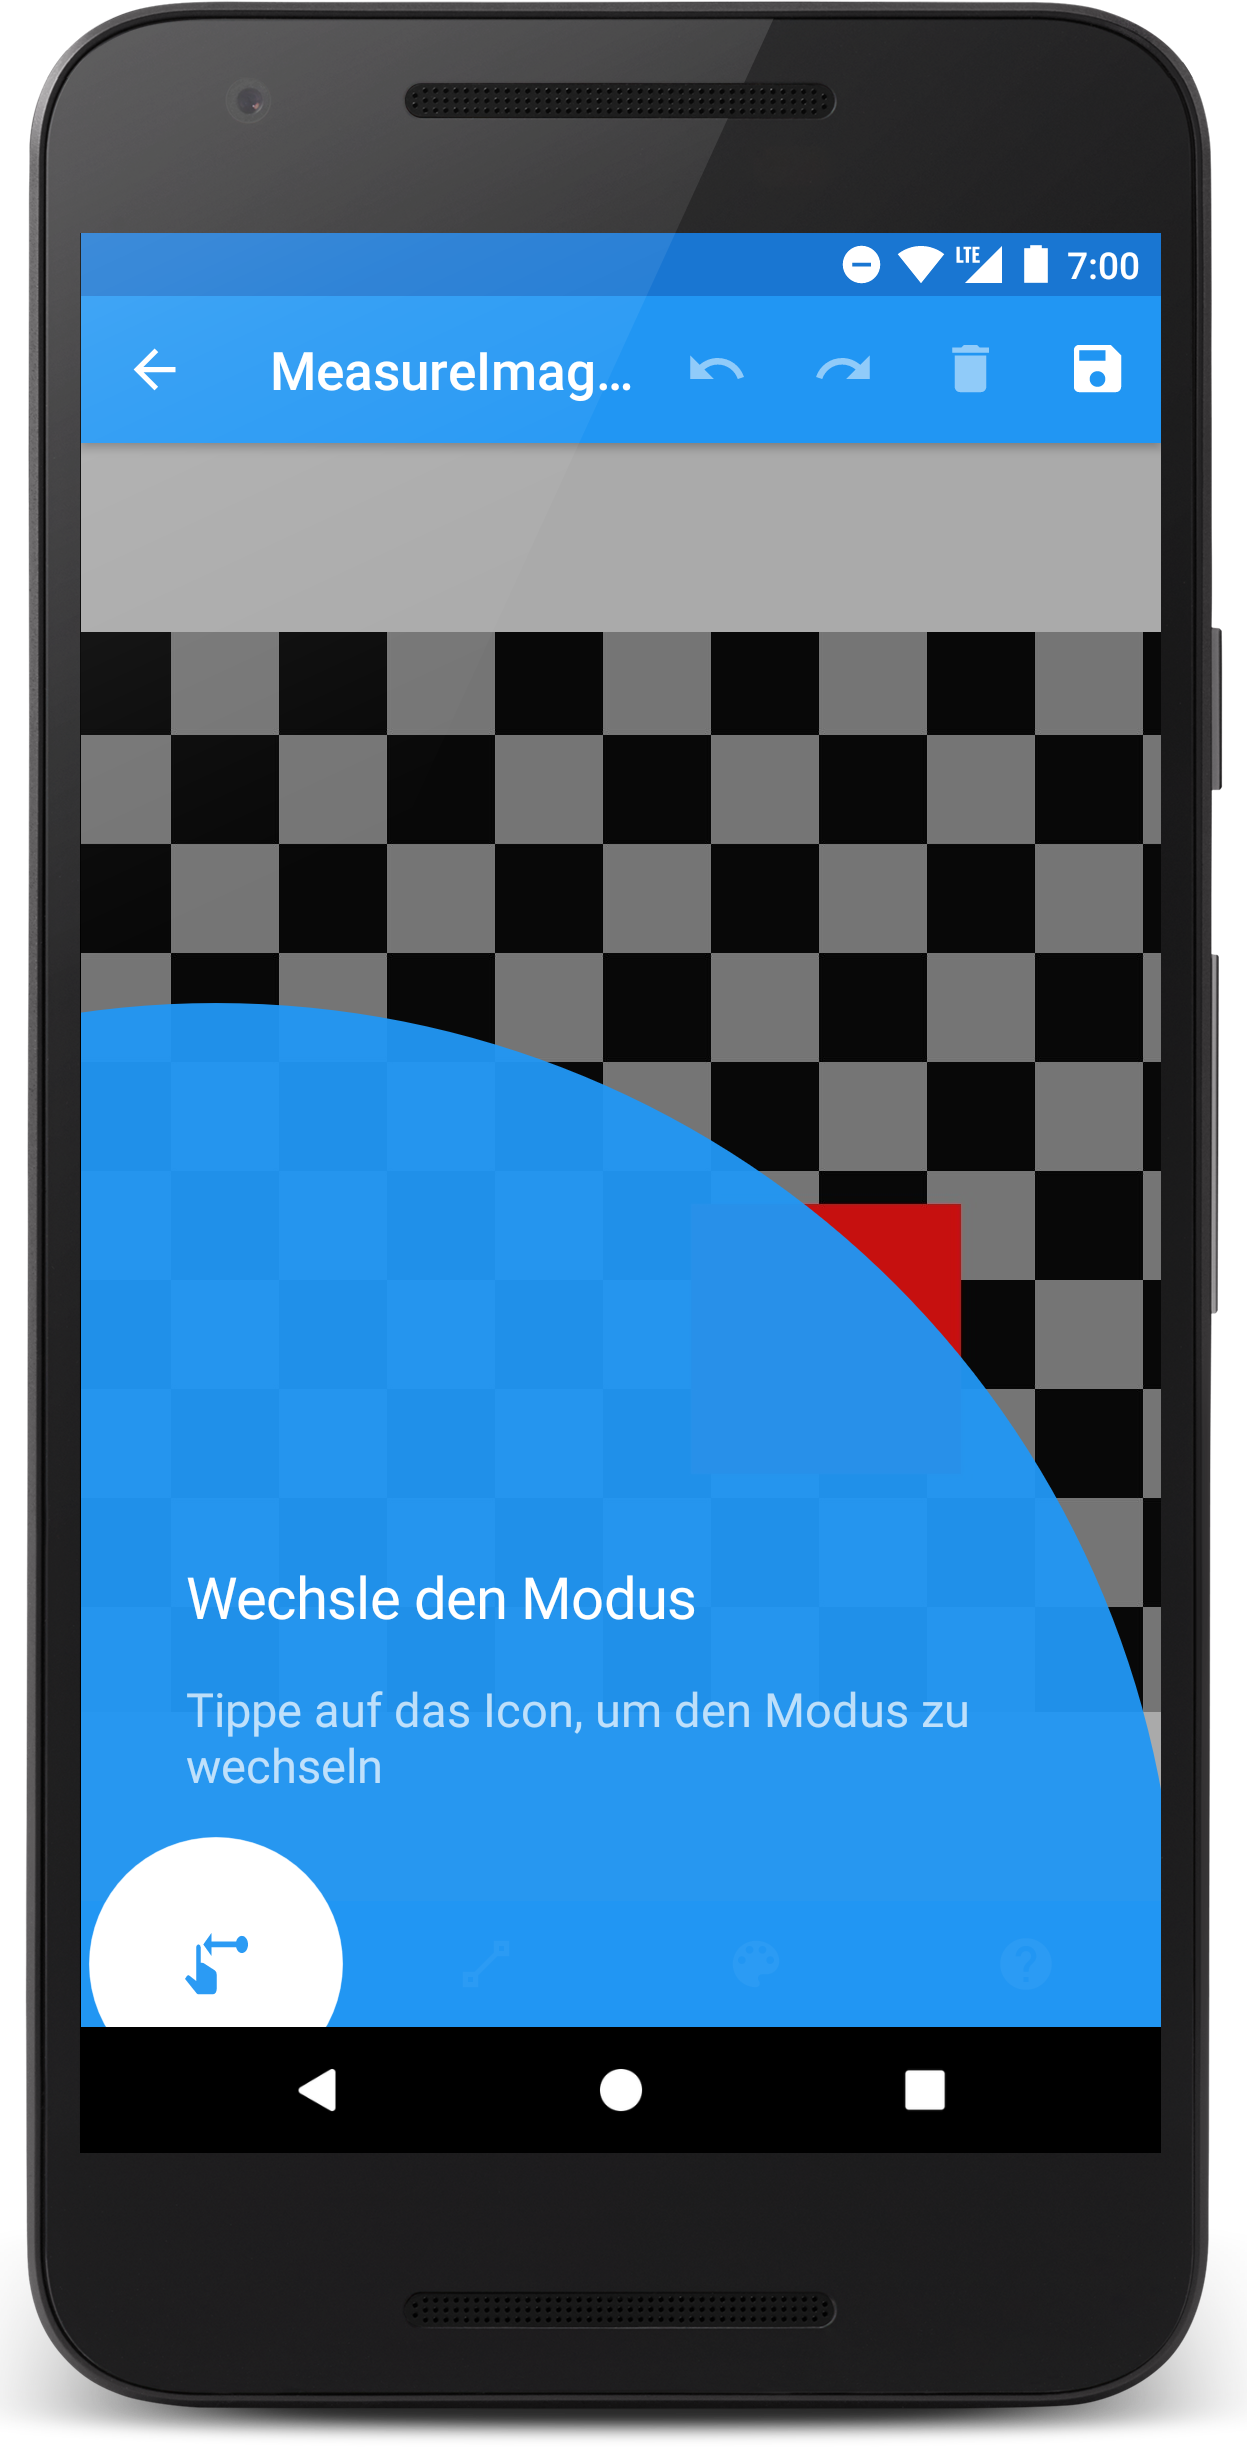
\includegraphics[keepaspectratio, width=\textwidth]{prototype3/help_mode}
    \caption{\emph{Tap-Target} beim initialen Start der App}
    \label{fig:helpmode}
  \end{subfigure}
  \begin{subfigure}[t]{0.3\textwidth}
    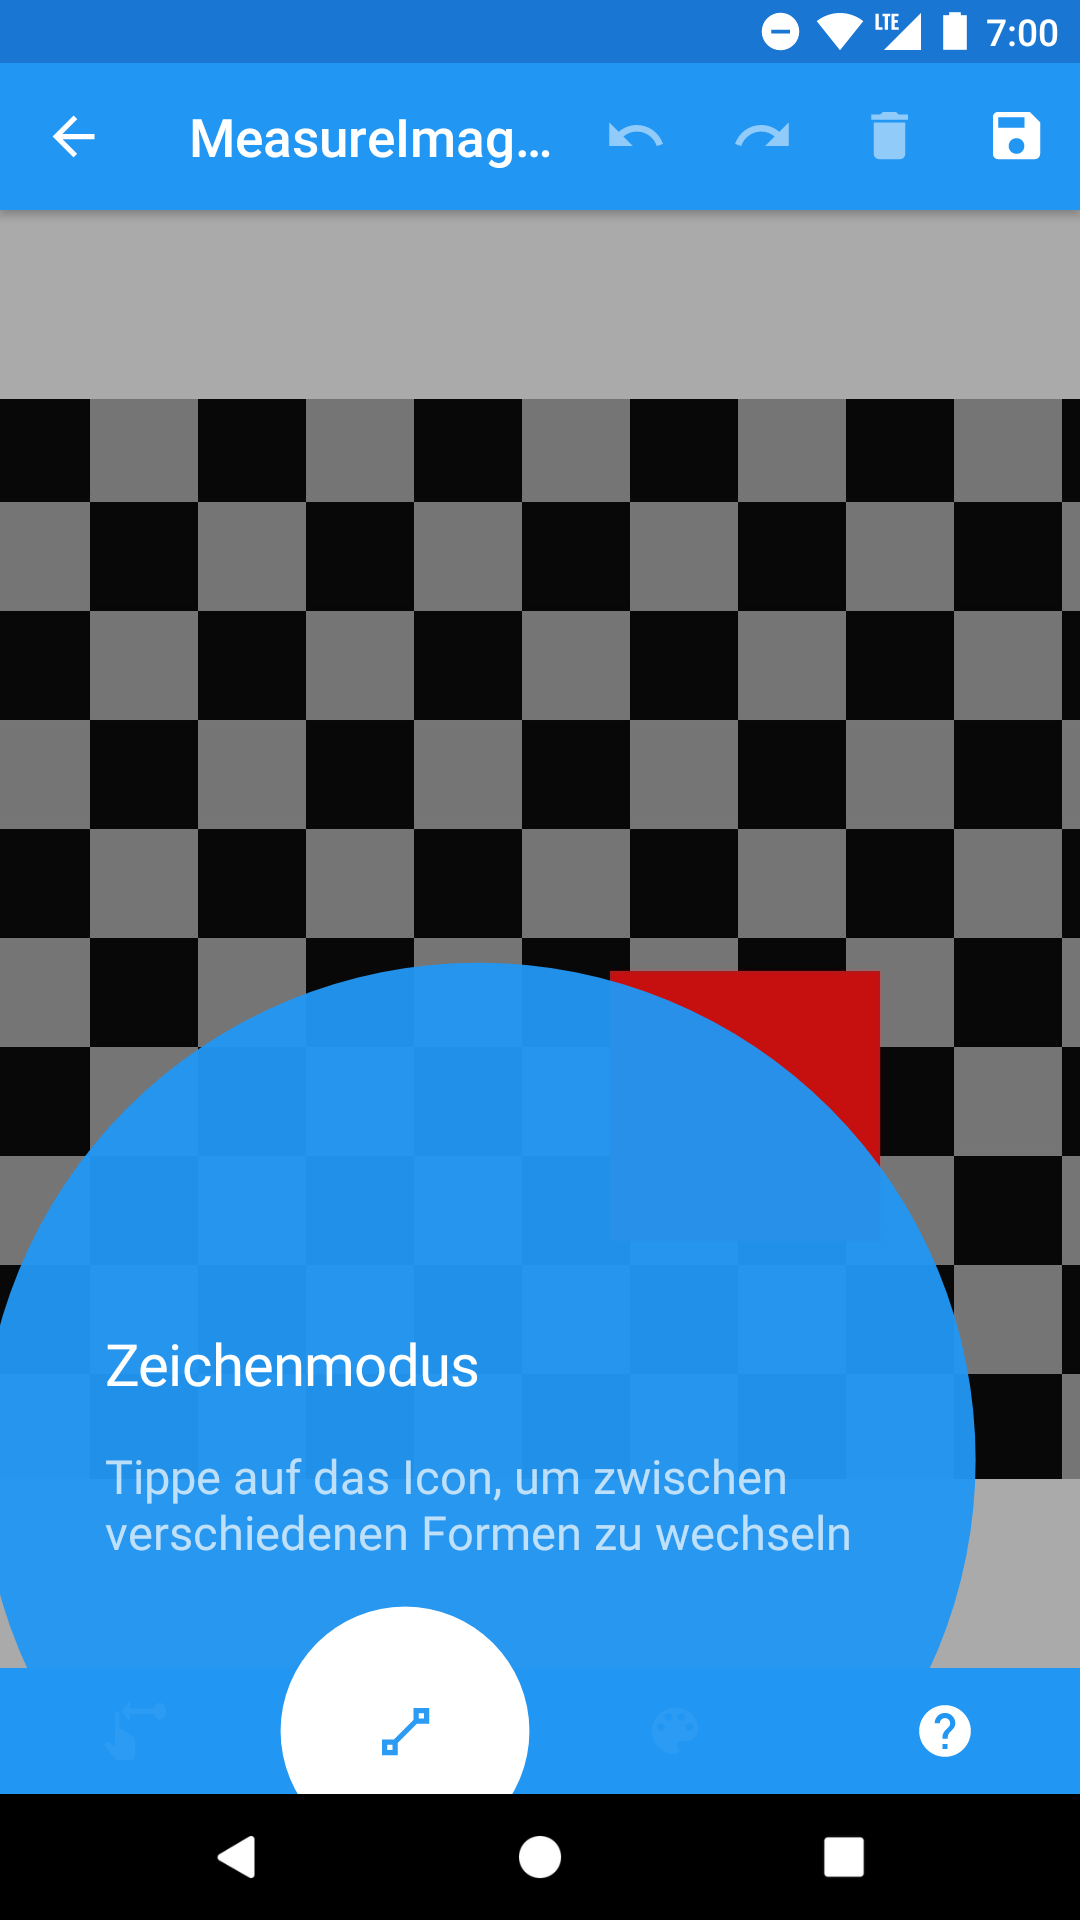
\includegraphics[keepaspectratio, width=\textwidth]{prototype3/help_draw}
    \caption{\emph{Tap-Target} beim initialen Wechsel in den Zeichen-Modus}
    \label{fig:helpdraw}
  \end{subfigure}
  \begin{subfigure}[t]{0.3\textwidth}
    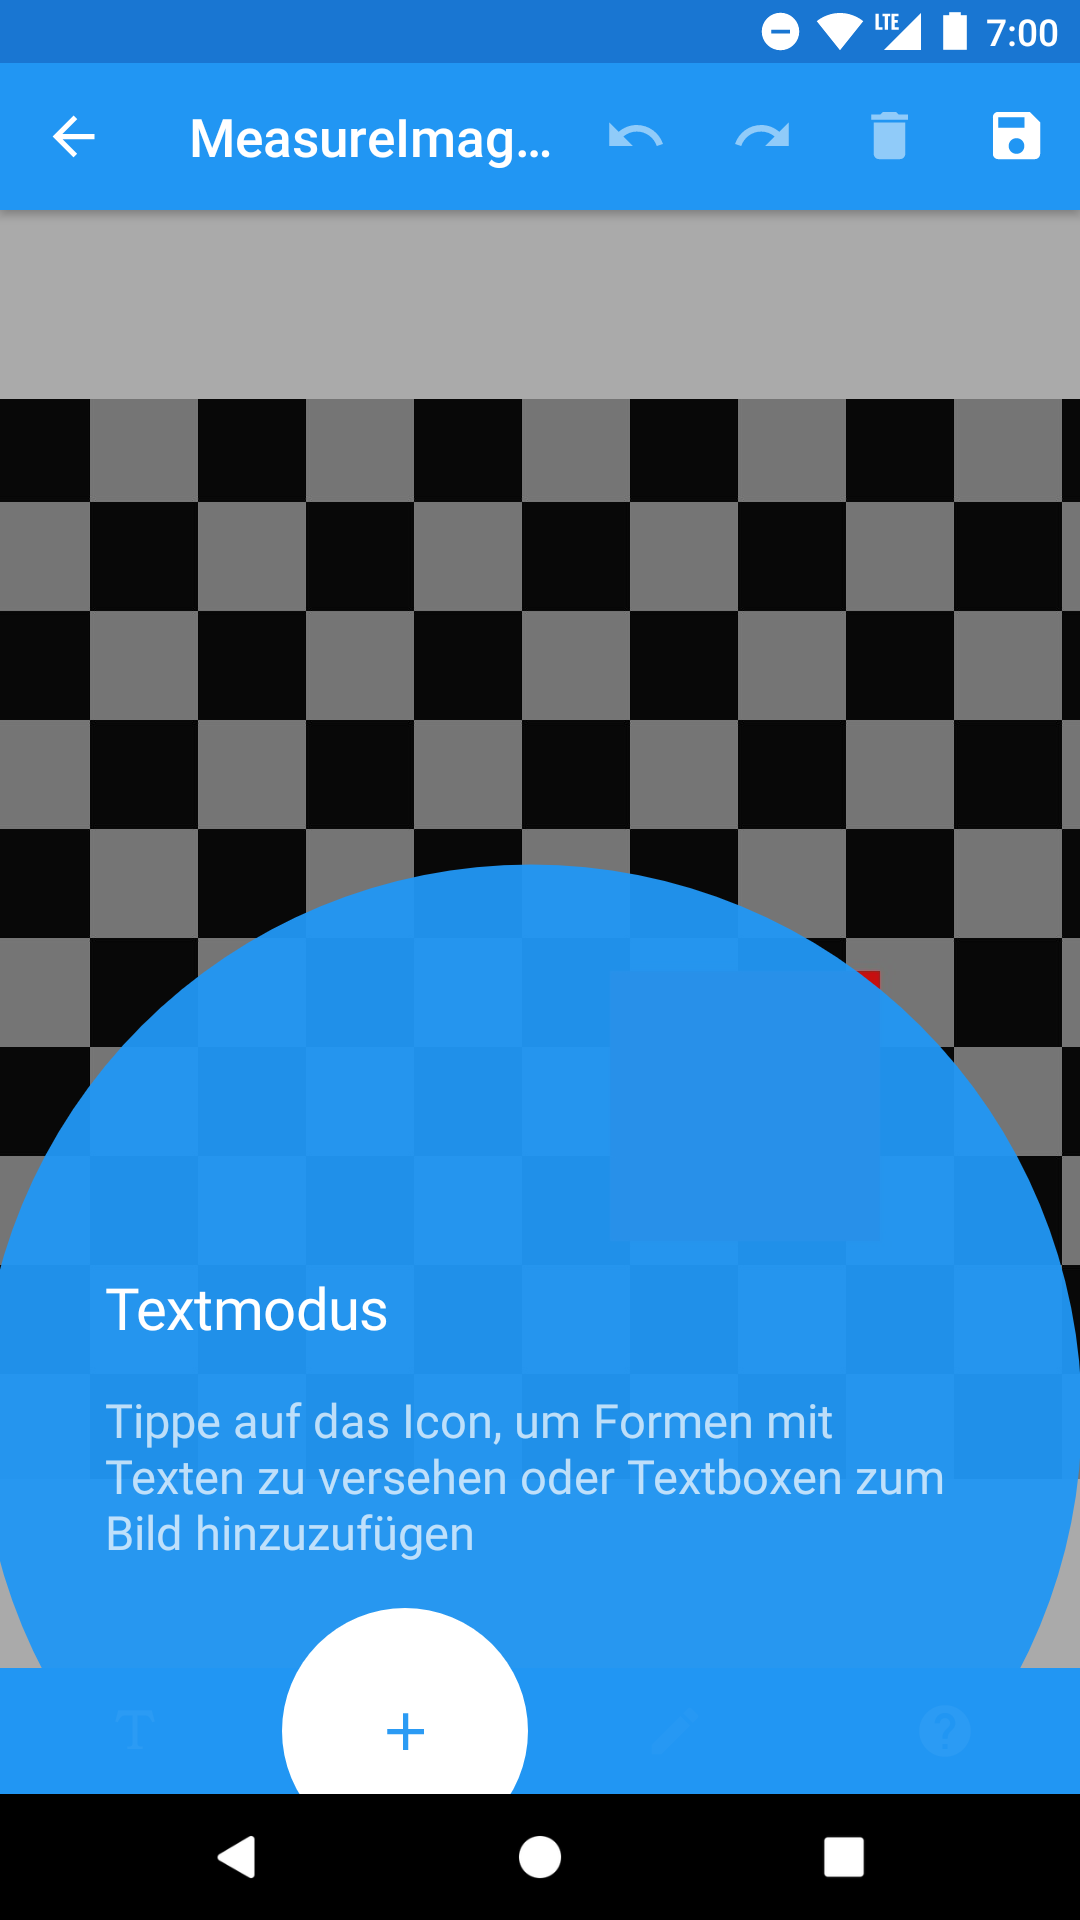
\includegraphics[keepaspectratio, width=\textwidth]{prototype3/help_text}
    \caption{\emph{Tap-Target} beim initialen Wechsel in den Text-Modus}
    \label{fig:helptext}
  \end{subfigure}
  \caption{Die drei verwendeten \emph{Tap-Targets} des dritten Prototyps}
  \label{fig:taptargets}
\end{figure}

Die verwendete \emph{Android-Library} für den Farbdialog\urlnote{https://github.com/jaredrummler/ColorPicker} verfügt bereits über einen ``Preset-Mode'', welcher es ermöglicht, anstatt des gesamten Farbkreises nur eine Farbpalette mit den häufigst genutzten Farben anzuzeigen.
Dieser ``Preset-Mode'' wurde als Standard ausgewählt, und wird beim Öffnen dies Dialogs angezeigt (siehe \autoref{fig:color3}).
Zusätzlich bietet sich dem Benutzer die Möglichkeit über den ``Custom''-Button unten links in die fortgeschrittene Ansicht (siehe \autoref{fig:color1}) zu wechseln. \\

\begin{figure}[h]
  \centering
  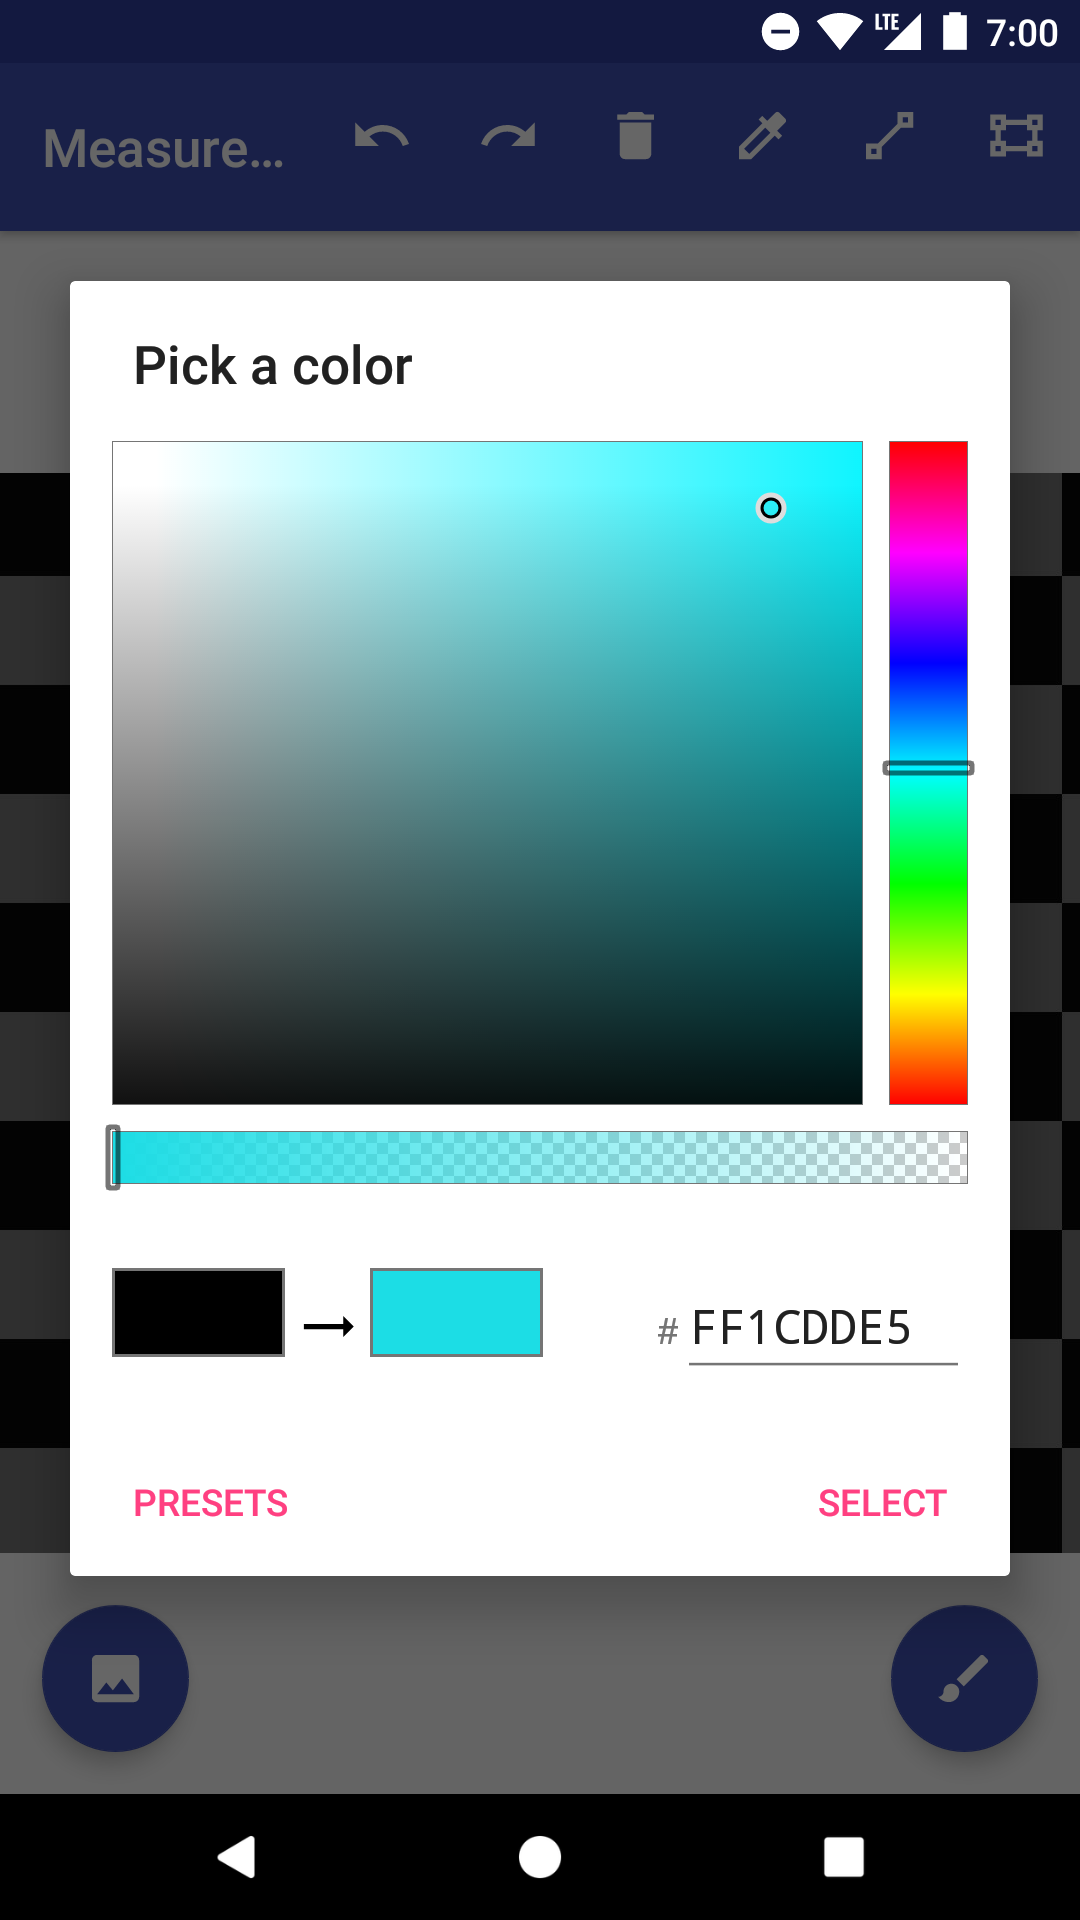
\includegraphics[keepaspectratio, width=0.4\textwidth]{prototype3/color}
  \caption{Vereinfachter Farbdialog des dritten Prototyps}
  \label{fig:color3}
\end{figure}

Um mit einem Gerüsttyp verlinkte Formen deutlicher zu kennzeichnen, wurde ein Lineal-Icon hinter die Indikator-Zahl gehangen (siehe \autoref{fig:indicator2}).
Dies soll dazu führen, dass der Nutzer beim Sehen des Indikators direkt den Gerüsttyp-Dialog assoziiert und die Indikator-Zahl nicht mit der Kantenbeschriftung verwechselt.
Zudem wurde in diesem Prototyp die Position des Indikators so verändert, dass dieser neben dem Text der eingetragenen Messwerten steht.
Dies soll verhindern, dass der Indikator einer falschen Form zugeordnet wird, falls Formen auf dem Bild nah nebeneinander liegen. \\

\begin{figure}[h]
  \centering
  \begin{subfigure}[t]{0.4\textwidth}
    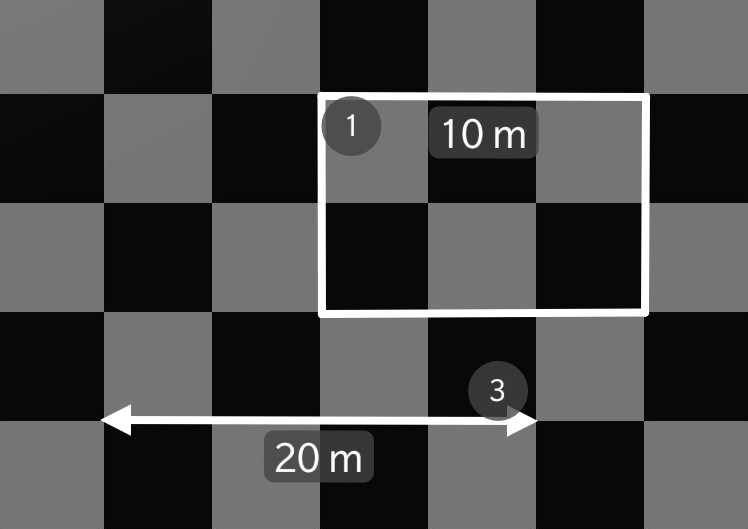
\includegraphics[keepaspectratio, width=\textwidth]{prototype3/indicator1}
    \caption{Gerüsttyp-Indikator im zweiten Prototyp}
    \label{fig:indicator1}
  \end{subfigure}
  \begin{subfigure}[t]{0.4\textwidth}
    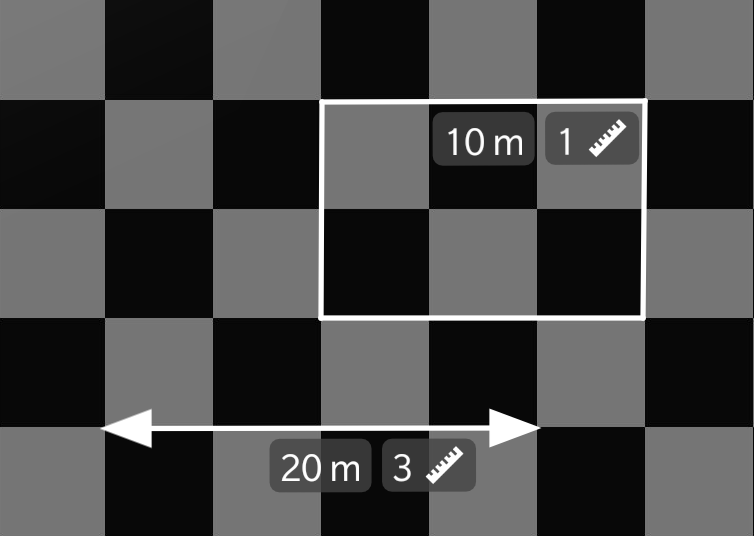
\includegraphics[keepaspectratio, width=\textwidth]{prototype3/indicator2}
    \caption{Gerüsttyp-Indikator im dritten Prototyp}
    \label{fig:indicator2}
  \end{subfigure}
  \caption{Vorher-Nachher-Vergleich des Gerüsttyp-Indikators}
  \label{fig:indicators}
\end{figure}

Im Gerüsttyp-Dialog wurden \emph{AutoCompleteTextField}-Elemente\urlnote{https://developer.android.com/reference/android/widget/AutoCompleteTextView.html} benutzt, welche die eingetragenen Messwerte der Form beim Tippen vorschlagen.
So hat der Nutzer direkt eine Übersicht über die zuvor eingetragenen Messwerte, und muss nicht zwischen Dialog und Bild wechseln. \\

Beide neuen Formen (vgl. \autoref{fig:indicator2}) sind durch Unterklassen, welche von der abstrakten Oberklasse \emph{MeasureShape} erben, modelliert und umgesetzt worden.
Dieser Prozess war für das Hinzufügen der Pfeil-Form trivial, da diese nahezu identisch zu der bereits vorhandenen Linien-Form ist.
Hier wurde lediglich beim Zeichnen der Form eine Pfeilspitze übersprungen.
Bei der Freitext-Form gab es jedoch ein paar Besonderheiten, die zu beachten waren:
Die Freitext-Formen werden im Gegensatz zu allen anderen Formen nicht mit Hilfe einer Zeichen-Geste auf das Bild gezeichnet, sondern sollen in der Mitte der derzeitigen Sichtbereichs erscheinen.
Zudem muss die Größe der Freitext-Form abhängig von der eingegebenen Textlänge dynamisch berechnet und beim Verändern erneut angepasst werden. \\

\section{Testing}\label{sec:test3}
Der dritte Prototyp war 8 Tage in den Arbeitsalltag der beiden Testpersonen integriert, bevor am 24. Januar 2018 Feedback zur Benutzung des Prototyps gesammelt wurde. \\

Die neuen Freitext-Form sei laut Aussage beider Testpersonen in ihrer Funktion nützlich, habe aber den Nachteil, dass wenn mehrere Text-Formen nebeneinander benutzt werden, das Bild schnell unübersichtlich werde. \\

Zudem sei der Dialog zum Speichern des Bildes irritierend, da sowohl im Dialog, als auch in der bestehenden App nach einer Beschreibung für das Bild gefragt wird.
Dies sei ``[\dots] lästig, weil man zweimal den selben Text eintippen muss'' (Testperson 1). \\

Ein weiterer Aspekt, der beiden Testpersonen augefallen ist, sei eine automatische Rotation von aufgenommenen Bildern.
Laut der Tester werden im Hochformat aufgenommene Bilder ins Querformat gedreht, obwohl sie in der Oberfläche zum Schneiden bzw. Rotieren nicht verändert wurden.

Diese drei Test-Ergebnisse sollen im nächsten Kapitel in einem vierten Durchlauf des \hcdp{} weiter untersucht und optimiert werden.
